\documentclass[10pt]{article}
\usepackage[a4paper,left=0.75in,right=0.75in,top=0.6in,bottom=0.6in]{geometry}
\usepackage{fontspec}
\setmainfont{Carlito}
\usepackage{xcolor}
\usepackage{enumitem}
\usepackage{booktabs}
\usepackage{tabularx}
\usepackage[hidelinks]{hyperref}
\definecolor{piccteal}{RGB}{20,148,145}
\pagestyle{empty}
\setlength{\parindent}{0pt}
\setlength{\parskip}{4pt}
\frenchspacing
\usepackage{graphicx}
\hyphenpenalty=10000
\exhyphenpenalty=10000
\tolerance=3000
\emergencystretch=2em
\setlist[itemize]{leftmargin=14pt,topsep=1pt,itemsep=2pt,parsep=0pt}
\setlist[enumerate]{leftmargin=16pt,topsep=1pt,itemsep=3pt,parsep=0pt}
\newcommand{\head}[1]{\vspace{3pt}{\color{piccteal}\bfseries\large #1}\par\vspace{1pt}}
\begin{document}
{\color{piccteal}\bfseries\LARGE Commercial brief: home care pricing and the 2026/27 fee round}\par
\vspace{2pt}
{\small Nihal Naresh Kumar, November 2026. Pay, on-cost, mileage and Bury Council rates are published figures; the contracts, homes, tender and supplier ledger are synthetic. Full model: \href{https://github.com/nihalgowda2002-arch/care-contract-pricing}{github.com/nihalgowda2002-arch/care-contract-pricing}.}

\head{Summary}
Costs on the portfolio rose 5.6\% in 2026/27: 3.9 points from the National Living Wage rise to \pounds12.71 and CPI on non-pay costs, and 1.8 points from HMRC's approved mileage rate rising from 45p to 55p, which was announced in May, after councils had set their fees. A 3.6\% uplift on every contract cuts the portfolio margin from 4.2\% to 2.3\%, about \pounds249,000 a year on \pounds12.2m of revenue. Council work, three quarters of revenue, moves from a margin of minus 0.5\% to minus 2.5\%, and NHS and self-funded work carry the profit.

\begin{center}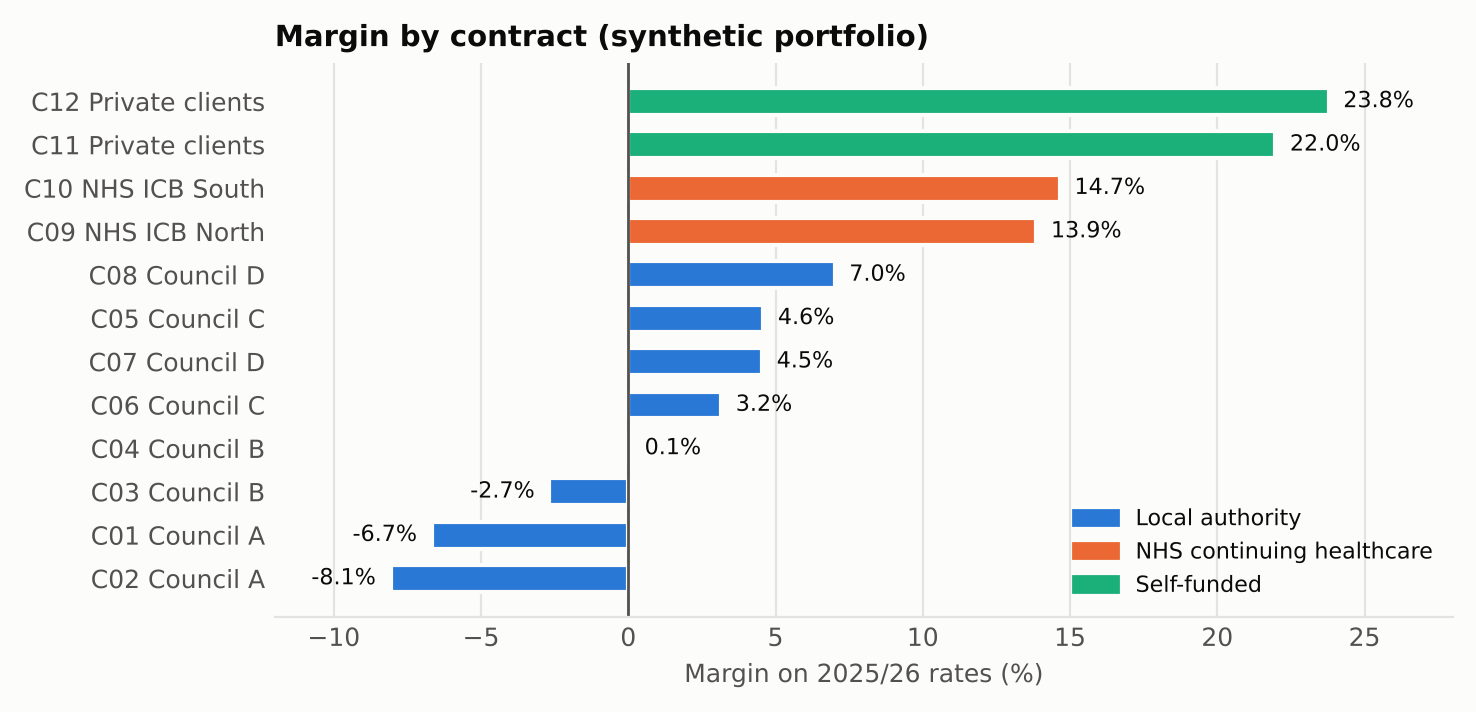
\includegraphics[width=0.74\linewidth]{fig2_contract_margins.png}\end{center}
\vspace{-8pt}

\head{What a contact hour costs (typical urban package, 2026/27)}
\begin{tabularx}{\linewidth}{Xrrrr}
\toprule
 & 15 min & 30 min & 45 min & 60 min \\
\midrule
Price per contact hour, urban (5\% margin) & \pounds41.04 & \pounds31.48 & \pounds28.30 & \pounds26.71 \\
Price per contact hour, rural & \pounds58.64 & \pounds40.28 & \pounds34.17 & \pounds31.11 \\
\bottomrule
\end{tabularx}

\vspace{2pt}
The package costs \pounds28.25 an hour and needs \pounds29.73 at a 5\% margin; care worker pay and on-costs are 76\% of cost. Bury's 2026/27 standard rate of \pounds24.30 covers the \pounds23.80 direct cost and 11\% of overheads, and its enhanced rate of \pounds28.53 leaves a margin of about 1\%. A 25\% change in travel time moves the price by \pounds1.36 an hour, slightly more than a 5\% change in pay.

\head{Recommendations}
\begin{enumerate}
\item \textbf{2027/28 fee submissions:} show the cost build-up line by line, and ask for the mileage increase as its own item, since 2026/27 fees did not include it. Contracts below the 5\% target need 6\% to 21\% to reach it; start with the council contracts that already lose money.
\item \textbf{Tender pricing:} price 15-minute and rural visits separately, or ask for a rural supplement; they cost 54\% and 28\% more per contact hour than 60-minute and urban 30-minute visits.
\item \textbf{Council E tender:} bid with conditions. The \pounds32.20 ceiling gives a 3.8\% margin at 40\% rural hours (walk-away rate \pounds31.61). Ask for a rural supplement or cap rural hours at 34\%, and phase the start, as 30 new care workers are needed against 24 we can recruit in time.
\item \textbf{Care homes:} Home 4 loses about \pounds75,600 a year at 82\% occupancy and breaks even at 86.6\%, about two more residents. Focus admissions there and review its council fee; Home 2 (2.9\% margin) is next.
\item \textbf{Purchasing:} move gloves, aprons and continence pads to the cheapest current supplier (\pounds12,300 a year) and recruit to replace 30\% of agency hours (\pounds56,600 a year): together 5.1\% of \pounds1.36m of spend.
\end{enumerate}

\head{Method and limits}
Visit costs combine contact, travel and training time at the National Living Wage, 12.07\% holiday accrual, employer National Insurance (15\% above \pounds5,000) and pension (3\% of qualifying earnings), mileage, branch staff (12\% of care worker cost) and non-pay overheads. Travel time, overheads and the visit mix are assumptions that a provider's rota and ledger data would replace. Sick pay, sleep-ins, enhancements and the Apprenticeship Levy are not modelled.
\end{document}
